\section{Solução}
O subsistema de Energia é responsável pela alimentação da Estação Coletora e pelo funcionamento do motor para o triturador . O subsistema se divide em dois, sendo o primeiro o do motor monofásico que será integrado com o subsistema de estrutura e eletrônica, garantindo o funcionamento do mesmo e a segurança da máquina e dos integrantes, e o segundo será da fonte simétrica que estará integrado com o subsistema de eletrônica, fornecendo a energia necessária para o funcionamento dos seus equipamentos.

\subsection{Motor Monofásico}
É um componente eletromecânico muito utilizado, devido a sua eficiência e simplicidade. São construídos para suprir a necessidade de movimento de rotação em situações onde é disponibilizada apenas uma única fase de corrente alternada. 
O motor monofásico, possui estator e rotor como qualquer outro atuador eletromagnético. Entretanto, por se tratar de um componente monofásico possui apenas um conjunto de bobinas, análogo a visão de apenas uma fase de um motor trifásico de indução. O motor monofásico utiliza o bobinamento para um rotor gaiola de esquilo.

\begin{figure}[!h]
	\centering
		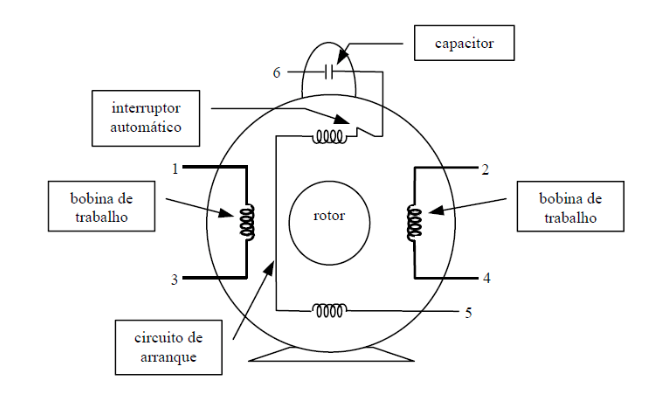
\includegraphics[scale=0.6]{figuras/energia/1.png}
	\caption{Detalhes de um motor monofásico.}
\end{figure}

O campo girante do motor monofásico possui certas particularidades como a necessidade de um enrolamento auxiliar para gerá-lo. Para inversão do sentido de giro desse tipo de motor, também é necessário um esquema que possa fazer com que sua partida se dê para outro lado. 

Para este projeto o motor escolhido, foi o de indução monofásico da WEG, que fará a alimentação principal do projeto. Atuando juntamente com o disjuntor para garantir a integridade do motor e de todos o sistema contra eventuais problemas no circuito. 

\begin{figure}[!h]
	\centering
		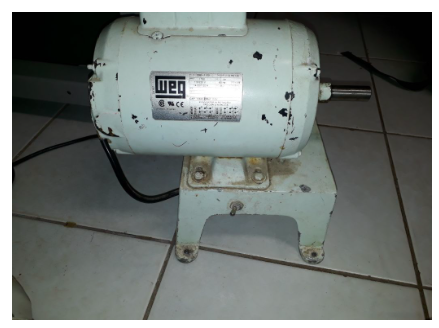
\includegraphics[scale=0.5]{figuras/energia/2.png}
	\caption{Motor de Indução Monofásico da WEG.}
\end{figure}

O motor fornecido para a Estação Coletora foi o WEG D56 monofásico. A seguir segue as  as seguintes especificações.

\begin{itemize}
    \item Potência = 0,75 kW / 1 cv
    \item Rotação = 1730 RPM
    \item Frequência = 60 Hz
    \item Corrente Nominal: 7,0 A (Para 220v)
    \item Fator de Serviço: 1,15
    \item Relação Corrente de Partida e Nominal = Ip/In = 5,5
    \item Tempo de Rotor Bloqueado: 10s (Frio) e 6s (Quente)
\end{itemize}

CREDER (2005) define a relação entre potência, conjugado e rotação de um motor elétrico como:

\begin{figure}[!h]
	\centering
		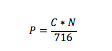
\includegraphics[scale=0.9]{figuras/energia/3.png}
	\caption{Fórmula 1}
\end{figure}

P = Potência em cv;

C = Conjugado em kgm;

N = Rotação em rpm;

Como o motor terá seu eixo acoplado com um redutor de 1:40, a rotação cairá de 1730 para 43,25 rpm.

\begin{figure}[!h]
	\centering
		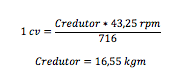
\includegraphics[scale=0.9]{figuras/energia/4.png}
	\caption{Fórmula 2}
\end{figure}

\subsubsection{Disjuntor}

O disjuntor é um dispositivo eletromecânico que tem a função de proteger as instalações elétricas, ou seja, assim que a corrente elétrica que passa por ele ultrapassa o seu valor nominal, ele interrompe o circuito impedindo o fornecimento de energia para as cargas do circuito, evitando assim que elas e o circuito danifiquem.

Possuem um dispositivo de interrupção da corrente constituído por lâminas de metais de coeficientes de dilatação térmica diferentes, soldados. A dilatação desigual das lâminas, por efeito do aquecimento, provocado por uma corrente de sobrecarga faz interromper a passagem de corrente no circuito.

O disjuntor atuará todas as vezes que houver pico de corrente, sobrecarga e curto-circuito, mas é importante destacar que para todos os disjuntores funcionarem corretamente é fundamental haver o correto dimensionamento do circuito e dos componentes.

Aplicando em nosso projeto o disjuntor escolhido foi o magnético, pois, possui a mesma função dos disjuntores eletromagnéticos e térmicos que é a proteção dos equipamentos elétricos contra os possíveis curtos-circuitos e as sobrecargas, mas tem uma vantagem quando comparado com os outros, que é a precisão maior para detectar o valor da corrente elétrica visando a segurança do sistema.

\begin{figure}[!h]
	\centering
		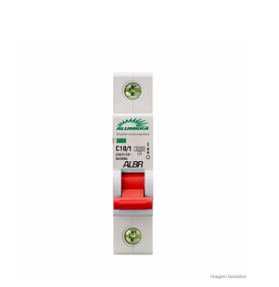
\includegraphics[scale=0.5]{figuras/energia/5.png}
	\caption{Disjuntor C10-1 Alumbra.}
\end{figure}

Para a realização do dimensionamento do disjuntor, precisamos saber a corrente de emprego (Ie) do sistema que é dada pela seguinte equação:

\begin{figure}[!h]
	\centering
		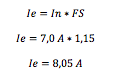
\includegraphics[scale=0.9]{figuras/energia/6.png}
	\caption{Fórmula 3}
\end{figure}

A corrente de partida é definida por:

\begin{figure}[!h]
	\centering
		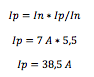
\includegraphics[scale=0.9]{figuras/energia/7.png}
	\caption{Fórmula 4}
\end{figure}

Observando os resultados encontrados,as curvas B,C e D e a norma ABNT NBR NM 60898, foi escolhido um disjuntor termomagnético C10, protegendo assim contra curtos circuitos e sobrecargas. Os disjuntores de curva C suportam uma corrente instantânea de 5 a 10 vezes maior que a corrente nominal, sendo suficiente para a corrente de partida do motor em questão. 

\subsection{Sistema de Frenagem por corrente contínua}
De forma clara, esse tipo de frenagem consiste em retirar a corrente alternada que alimenta o motor e ao mesmo tempo injetar uma corrente contínua, fazendo com que ocorra a parada do mesmo. 

Isso acontece devido ao envio de uma corrente contínua para o enrolamento estatórico, e assim estabelece um fluxo magnético estacionário cuja curva tem uma distribuição fundamental de forma senoidal. Com isso, a rotação do rotor em seu campo gera um fluxo de corrente alternada no mesmo, o qual também estabelece um campo magnético estacionário com respeito ao estator. Devido à interação do campo magnético resultante e da corrente rotórica, o motor desenvolve um torque de frenagem cuja magnitude depende da intensidade do campo, da resistência do circuito rotórico e da velocidade do rotor.

Na prática, isso foi realizado a partir de uma ponte retificadora, sendo ela o principal componente do sistema de frenagem.

\subsubsection{Ponte Retificadora}
Os circuitos retificadores são circuitos elétricos elaborados para a conversão de corrente alternada em contínua para alimentação de uma gama de equipamentos, sendo no nosso caso, aplicados a placas de circuito eletrônicos e a injeção de corrente no motor para a frenagem. 

Os retificadores que aproveitam as duas metades da onda CA são chamados de retificadores de onda completa e são podem ser diodos e tiristores, além de um transformador.

A usada nos dois casos, serão as pontes retificadoras compostas por um banco de diodos. Eles têm como função conduzir corrente elétrica em um único sentido ou fluxo, permitindo assim a passagem de corrente em um único sentido. É composto por dois terminais, o ânodo e o cátodo. 

A polarização direta acontece quando o pólo positivo da fonte entra em contado com o ânodo do diodo, ou seja, na polarização direta o diodo permite a passagem de corrente elétrica. O diodo permite que apenas a parte positiva da senóide da fonte alternada passe pelo circuito, dessa maneira, convertendo o sinal para contínuo. Da mesma forma ocorre quando o polo negativo da fonte entra em contato com o cátodo do diodo, com a diferença que a parte negativa da senóide é convertida para contínua.

\begin{figure}[!h]
	\centering
		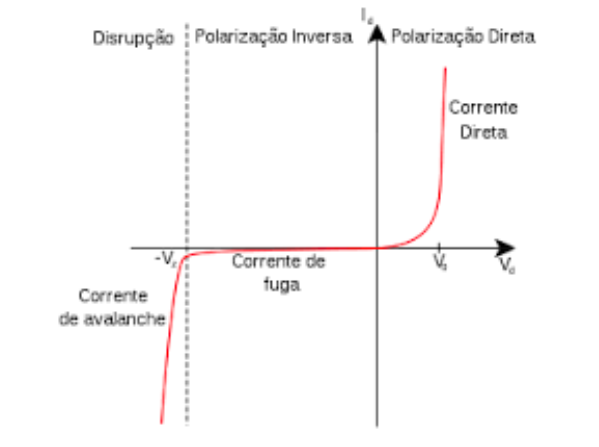
\includegraphics[scale=0.4]{figuras/energia/8.png}
	\caption{Polarização Direta.}
\end{figure}

O diodo funciona como uma chave, após o fornecimento de uma corrente alternada, a chave se comporta de duas maneiras, sendo ela fechada (resistência zero) para uma polaridade da tensão de entrada e como uma chave aberta (resistência infinita) para a polaridade oposta. E como sua função é alterar a corrente, ele faz com que a corrente passe em apenas uma polaridade. O gráfico mostra a tensão de chegada no diodo.

\begin{figure}[!h]
	\centering
		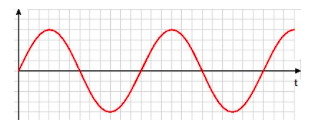
\includegraphics[scale=0.5]{figuras/energia/9.png}
	\caption{Tensão de entrada do diodo oscilando entre o positivo e o negativo.}
\end{figure}

Após passar pelo diodo a tensão passa a ter apenas uma polaridade, como mostra o gráfico 2.

\begin{figure}[!h]
	\centering
		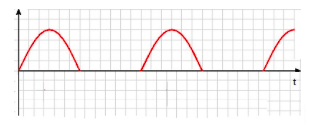
\includegraphics[scale=0.5]{figuras/energia/10.png}
	\caption{Tensão de saída do diodo meia onda.}
\end{figure}

E seguindo a mesma lógica, após passar pela ponte retificadora e por um filtro capacitivo,  a tensão começa a se linearizar.

\begin{figure}[!h]
	\centering
		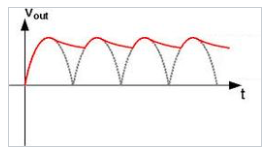
\includegraphics[scale=0.5]{figuras/energia/11.png}
	\caption{Sinal senoidal de saída pós filtro capacitivo}
\end{figure}

A ponte retificadora do sistema de frenagem trabalhará em tensão 220V. Foi realizada medição da resistência do estator do motor, sendo de 25 ohms. Aplicando a Lei de Ohm temos.

\begin{figure}[!h]
	\centering
		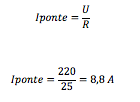
\includegraphics[scale=0.9]{figuras/energia/12.png}
	\caption{Fórmula 5}
\end{figure}

Concluímos então, que a ponte retificadora injetará 8,8 amperes de corrente contínua no motor para a realização da frenagem. Segundo o fabricante, o motor suporta a corrente de rotor bloqueado, ou seja, a corrente de partida (38,5 Amperes), por 6 segundos. Sendo assim, foi escolhida a ponte KBPC1010 para o projeto, suportando tensão de até 1000V e corrente de 10 amperes.

\subsection{Fonte simétrica}
A fonte simétrica é muito utilizada  quando se necessita de tensões positivas e negativas na alimentação de circuitos com amplificadores operacionais. 

Para a integração com o subsistema de eletrônica uma fonte simétrica será necessária, com potência de 50W e saídas de 5V e 12V DC, para fazer a alimentação dos componentes de alimentação externa do sistema.

\subsubsection{Transformador}
Transformadores são dispositivos capazes de aumentar ou reduzir valores de tensão. Com funcionamento baseado da Lei de Lenz e na Lei de Faraday. É constituído por um núcleo, feito de um material altamente magnetizável, e duas bobinas com número diferente de espiras isoladas entre si, a que recebe a tensão da rede chamada de primário, e a que tensão já sai transformada chamada de secundário.

O seu funcionamento é baseado na criação de uma corrente induzida no secundário, a partir da variação de fluxo gerada pelo primário. As tensões de entrada e saída são relacionadas ao número de espiras em casa bobina.

Baseado nessa relação considera-se que o transformador reduz a tensão se o número de espiras do secundário for menor que o número de espiras do primário e vice-verso.

Neste projeto o transformador é  um dos componentes da fonte simétrica responsável por fazer a integração entre o subsistema de energia com o da eletrônica para fazer a alimentação final do sistema.. Para esta fonte o transformador escolhido é um com trafo de 12V+12V e 5A para conseguir fazer a alimentação correta dos equipamentos eletrônicos com potência de 50W.

\begin{figure}[!h]
	\centering
		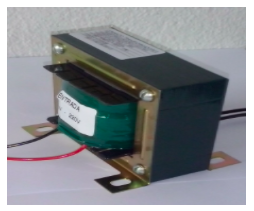
\includegraphics[scale=0.6]{figuras/energia/13.png}
	\caption{Transformador}
\end{figure}

\subsubsection{Capacitores}
Capacitores podem apresentar dois comportamentos quando ligados a fontes de tensão em um circuito. Caso o mesmo esteja alimentado por uma fonte de tensão contínua, ele armazenará energia entre suas placas até que sua tensão se iguale a da fonte, após carregado não passará mais corrente pelo capacitor. Diferente acontece quando a fonte fornece uma tensão alternada, nessa situação o capacitor alternará entre momentos onde armazena energia e momentos onde libera energia para o circuito, passando assim corrente pelo componente a todo instante.

O conceito de impedância é usado para facilitar a análise do circuito alimentado por tensão alternada, pois transforma um valor que depende da variação do tempo, e usa derivadas, em um número complexo (reatância capacitiva para capacitores e reatância indutiva pra indutores).

A impedância é a resistência do circuito a corrente alternada. Para calcular, é necessário o valor dos resistores e as impedâncias dos capacitores e indutores.

\begin{equation}
    Q = C \ast V
\end{equation}

Onde:

\begin{itemize}
    \item Q é a quantidade de cargas (coulombs);
    \item C é a capacitância (farads);
    \item V é a tensão entre as armaduras (V);
\end{itemize}

A quantidade de energia armazenada, por outro lado é dada por:

\begin{figure}[!h]
	\centering
		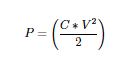
\includegraphics[scale=0.9]{figuras/energia/14.png}
	\caption{Fórmula 6}
\end{figure}

\begin{itemize}
    \item P é a energia armazenada em joules;
    \item C é a capacitância em farads;
    \item V é a tensão em volts;
\end{itemize}

Como iremos usar os capacitores com intuito de linearizar a tensão, o cálculo de dimensionamento do mesmo é feito da seguinte forma:

\begin{itemize}
    \item Temos que analisar a tensão de entrada, e como terá a queda de tensão provocada pelo transformador, a tensão de entrada no transformador será por volta de 
    
    Vc = 24rms = 33,94V
    \item O ripple que assumimos foi de 10\% 
    \begin{itemize}
        \item Vond = 10\% Vc
        \item Vond = 3,394 V
    \end{itemize}
\item Consideramos como carga todos os componentes que iremos alimentar, totalizando uma resistência equivalente de 89,8 omega.
    \item Feito isso, pela de Ohm encontramos a corrente que passará em nosso capacitor e assim podemos encontrar sua capacitância usando a seguinte fórmula
    
    C = I(Vc \* F)
    C = 0,37(33,94 \* 60)
    C = 185,5 microF
\end{itemize}

Usaremos um capacitor com uma maior capacitância afim de linearizar melhor nossa corrente.

\subsubsection{Step Down}
Step down é um dispositivo que permite regular a tensão requerida, é conhecido como módulo conversor de tensão e composto pelo regulador chaveado LM317, que trabalha com tensões de entrada entre 4,2V a 40V, oferecendo tensões de saída de 1,2V a 37V que podem ser ajustadas conforme a tensão necessária, através do trimpot que encontra-se na parte superior da placa.
Para correto funcionamento desse dispositivo é necessário observar a diferença de tensão de entrada de 1,5V maior que a de saída. A corrente normal de operação é aproximada de 2,2A, porém o módulo é capaz de reduzir uma carga de até 3A com ótima eficiência.
Vai atuar em conjunto com transformador, e capacitores na fonte simétrica, tendo a responsabilidade de filtrar a tensão de saída, oferecendo tensões de saídas estabilizadas.. Disponibilizará as tensões de 12V para 2A e de 5V para 2,8A para alimentação dos componentes eletrônicos requeridos.

\begin{figure}[!h]
	\centering
		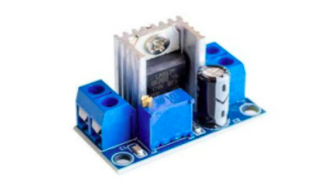
\includegraphics[scale=0.5]{figuras/energia/15.png}
	\caption{Módulo conversor de tensão LM317.}
\end{figure}

\subsection{Fios}
Os fios são condutores em formato cilíndrico que permitem passagem de corrente através de um condutor, sendo eles comumente feitos de alumínio ou cobre revestidos de material isolante como borrachas e PVC.

A seção transversal perpendicular de um fio elétrico deve ser projetado a fim de que com a passagem de corrente na fiação não seja comprometida. Quanto maior a passagem de corrente maior deve ser a bitola do fio, pois existe o risco de superaquecimento do material condutor do fio e caso ocorra, irá danificar o circuito. Então o tamanho de bitolas para baixas tensões é tabelado e padronizado para que seja feita com segurança as instalações nos equipamentos.

De acordo com a NBR 5410 que dita as normas para instalações elétricas em baixa tensão há uma padronização de fios de acordo com a quantidade de corrente requerida.

\begin{figure}[!h]
	\centering
		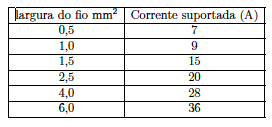
\includegraphics[scale=0.7]{figuras/energia/16.png}
	\caption{Tamanho requerido dos fios.}
\end{figure}

Aplicando em nosso projeto, consideramos que componente estejam a operar em sua maior capacidade, com suas as correntes máximas atingidas estarão dentro de uma margem confortável (corrente de emprego de 8 A e corrente ponte retificadora de 8,8 A) e considerando a seção mínima definida pela norma para circuitos de força, foi utilizado os condutores de 2,5 mm.

\subsection{Testes e Simulações}
Em um primeiro momento, foi realizada a simulação da possível solução para o circuito de acionamento do motor utilizando o software CADe-SIMU, testando os circuitos de potência e comando. A imagem abaixo apresenta a solução, onde:

\begin{itemize}
    \item RT: Relé Térmico
    \item V: Ponte Retificadora
    \item T1: Transformador
    \item S0: Acionamento Frenagem
    \item S1: Acionamento Motor 
\end{itemize}

\begin{figure}[!h]
	\centering
		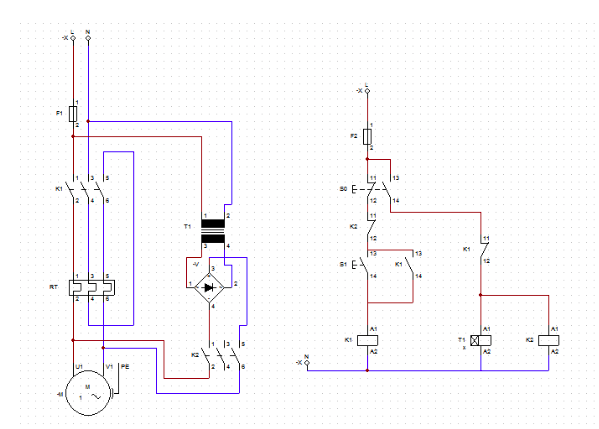
\includegraphics[scale=0.8]{figuras/energia/17.png}
	\caption{Simulação do circuito de comando e de força}
\end{figure}

A solução se baseia em utilizar duas contatoras, sendo uma para o acionamento do motor e outra para o acionamento do freio. Quando o selo de K1 for fechado, acionando então o motor, a contatora K2 mantem-se aberta. Ao se abrir K1, K2 é fechado, com isso é injetado corrente contínua no motor para sua frenagem. O tempo de trabalho do freio é controlado por um relé temporizador. 

Por questões de praticidade e custo benefício, a solução apresentada acima não será implementada. O subsistema de energia desenvolveu um código e através do uso de um Arduino  passou a ter um novo comando do acionamento do motor e de sua frenagem. 

\begin{figure}[!h]
	\centering
		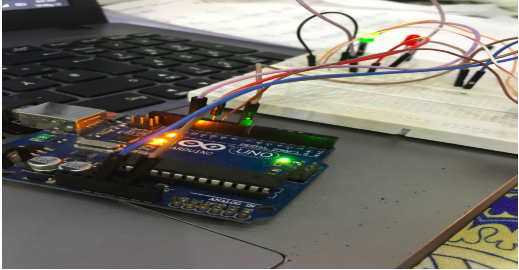
\includegraphics[scale=0.4]{figuras/energia/18.png}
	\caption{Teste com Arduino}
\end{figure}

O novo comando de acionamento se baseia na substituição de contatoras por relés. Sendo assim, não é mais necessário o uso de relé temporizador, contatos auxiliares, além das próprias contatoras, gerando grande economia. O controle dos relés se dá por meio do arduino, onde um relé será para o acionamento do motor, enquanto o segundo será para acionamento do freio, estando os dois em paralelo. O código foi desenvolvido para assim que o acionamento do motor for interrompido, imediatamente o segundo relé é acionado, ligando assim o freio de corrente contínua por tempo determinado, gerando uma parada do motor.